\documentclass[12pt]{article}
\usepackage{amsmath}
\usepackage{amssymb}
\usepackage{graphicx}
\usepackage{physics}
\usepackage{siunitx}
\usepackage{wrapfig}

\AtBeginDocument{\RenewCommandCopy\qty\SI}

\begin{document}
    \DeclareSIUnit{\cal}{cal}
    \DeclareSIUnit{\Cal}{Cal}
    \DeclareSIUnit{\calorie}{cal}
    \DeclareSIUnit{\Calorie}{Cal}
    

    \section{Question 4}
        \begin{wrapfigure}{r}{0.5\textwidth}
            \vspace{-30pt}
            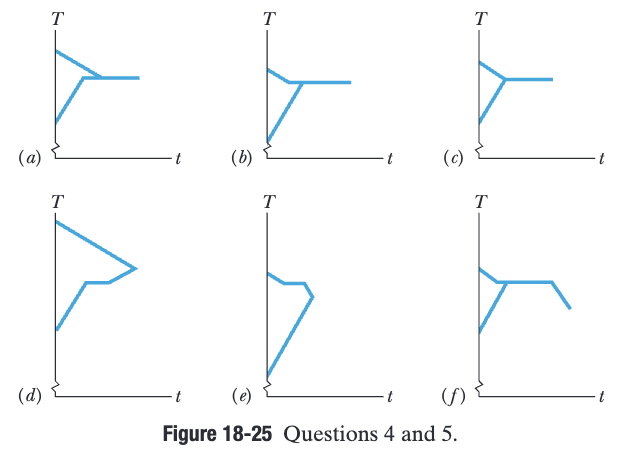
\includegraphics[width=0.5\textwidth]{picture_18-25.png} 
            % \label{fig:wrapfig}
        \end{wrapfigure}
        A sample A of liquid water and a sample B of ice, of identical mass, are placed in a thermally insulated container and allowed to come to thermal equilibrium. Figure 18-25$a$ is a sketch of the temperature T of the samples versus time t. (a) Is the equilibrium temperature above, below, or at the freezing point of water? (b) In reaching equilibrium, does the liquid partly freeze, fully freeze, or undergo no freezing? (c) Does the ice partly melt, fully melt, or undergo no melting?

    \subsection{Solution}

    \pagebreak
    \section{Question 5}
        Question 4 continued: Graphs b through f of Fig. 18-25 are additional sketches of T versus t, of which one or more are impossible to produce. (a) Which is impossible and why? (b) In the possible ones, is the equilibrium temperature above, below, or at the freezing point of water? (c) As the possible situations reach equilibrium, does the liquid partly freeze, fully freeze, or undergo no freezing? Does the ice partly melt, fully melt, or undergo no melting?

    \subsection{Solution}

    \pagebreak
    \section{Problem 5}
        At what temperature is the Fahrenheit scale reading equal to (a) twice that of the Celsius scale and (b) half that of the Celsius scale?

        \subsection{Solution (a)}
            This is totally algebraic. 
            The formula from fahrenheit to celsius is $T_F = \frac{9}{5}T_C + 32^{\circ}$.
            To convert between the two, we need to set $T_F$ and $T_C$ to be equal.
            \begin{align}
                T_F &=  \frac{9}{5}T_F + 32^\circ\\
                \frac{4}{5}T_F  &=  -32^\circ\\
                T_F &=  \boxed{-40^\circ}
            \end{align}

        \subsection{Solution (b)}
            This is also algebraic.
            The Fahrenheit reading is half that of the Celsius scale reading.
            \begin{equation}
                T_F = \frac{1}{2}T_C \leftrightarrow 2 T_F = T_C
            \end{equation}

            We can substitute this into the conversion formula we used in part (a).
            \begin{align}
                T_F &=  \frac{9}{5}T_C + 32^\circ\\
                    &=  \frac{18}{5}T_F + 32^\circ\\
                \frac{13}{5}T_F &=  -32^\circ\\
                T_F &=  \boxed{-\frac{160}{13}^\circ \approx -12^\circ}
            \end{align}

            We can verify this.
            \begin{align}
                T_F &=  \frac{9}{5}T_C + 32^\circ\\
                T_C &=  \frac{5}{9}\left(T_F - 32^\circ\right)\\
                    &=  \frac{5}{9}\left(-\frac{160}{13}^\circ - 32^\circ\right)\\
                    &=  \frac{5}{9}\left(-\frac{576}{13}^\circ\right)\\
                    &=  -\frac{320}{13} = 2 * T_F\ \ \ \checkmark
            \end{align}


    \pagebreak
    \section{Problem 7}
        Suppose that on a linear temperature scale X, water boils at $-53.5$°X and freezes at $-170$°X. What is a temperature of 340 K on the X scale? (Approximate water's boiling point as 373 K.)

        \subsection{Solution}
            We can put together a fraction of differences here to get a ratio of Kelvin to X scale.
            I will be approximating water's freezing point at 273 K.
            \begin{gather}
                \frac{T_X}{T_K} =   \frac{-53.5 + 170}{373 - 273} = \frac{116.5}{100} = \frac{233}{200} = 1.165 \frac{^\circ X}{K}
            \end{gather}

            Now, we can test the difference in temperature between the freezing point and 340 K.
            \begin{gather}
                \Delta T    =   340 \unit{\kelvin} - 273 \unit{\kelvin} = 67 \unit{\kelvin}
            \end{gather}

            Multiplying this by the ratio of \textdegree X to Kelvin, we get the difference in X between the target temperature and the freezing point.
            \begin{gather}
                67 \unit{\kelvin} * \frac{233^\circ X}{200 \unit{\kelvin}} = \frac{15611}{200} ^\circ X = 78.055 ^\circ X
            \end{gather}

            Add this to the freezing point to get the target value.
            \begin{gather}
                -170 ^\circ X + 78.055 ^\circ X = \boxed{-91.945 ^\circ X}
            \end{gather}

    \pagebreak
    \section{Problem 9}
        A circular hole in an aluminum plate is 2.725 \unit{\centi\meter} in diameter at 0.000\unit{\celsius}. What is its diameter when the temperature of the plate is raised to 100.0\unit{\celsius}?

        \subsection{Solution}
            For any given linear dimension, the expansion is defined by a formula using the coefficient of linear expansion $\alpha$.
            \begin{equation}
                \Delta L = L\alpha \Delta T
            \end{equation}

            We are working with aluminium, so $\alpha = 23 \times 10^{-6}/\unit{\celsius}$. 
            Also given the temperature change of 100\unit{\celsius} and an initial diameter of $27.25 \times 10^{-3} \unit{\meter}$, we can calculate the change in diameter. 
            \begin{align}
                \Delta L    &=  (27.25 \times 10^{-3} \unit{\meter})(23 \times 10^{-6}/\unit{\celsius})(100 \unit{\celsius})\\
                    &=  6.2675 \times 10^{-5} \unit{\meter}
            \end{align}

            Adding $\Delta L$ to $L$, we get our final answer and length.
            \begin{align}
                L_f &=  L_i + \Delta L\\
                    &=  27.25 \times 10^{-3} \unit{\meter} + 6.2675 \times 10^{-5} \unit{\meter}\\
                    &=  \boxed{27.31 \times 10^{-3} \unit{\meter}}
            \end{align}

    \pagebreak
    \section{Problem 11}
        What is the volume of a lead ball at 30.00\unit{\celsius} if the ball's volume at 60.00\unit{\celsius} is 50.00 \unit{\centi\meter^3}?
        
        \subsection{Solution}
            This is a similar problem to Problem 9 (5). 
            The coefficient of volume expansion is equal to thrice the coefficient of linear expansion, the latter of which for lead is $29 \times 10^{-6}/\unit{\celsius}$.
            This leaves the coefficient of volume expansion as $\beta = 3 * 29 \times 10^{-6}/\unit{\celsius} = 87 \times 10^{-6}/\unit{\celsius}$.
            We can in turn use this to find the change in volume.
            \begin{align}
                \Delta V    &=  V_i \beta \Delta T\\
                    &=  (50 \unit{\centi\meter^3}) (87 \times 10^{-6}/\unit{\celsius}) (30 \unit{\celsius})\\
                    &=  130.5 \times 10^{-3} \unit{\centi\meter^3}
            \end{align}

            Add the change to the initial value to get the final value.
            \begin{align}
                V_f &=  V_i + \Delta V\\
                    &=  50.0 \unit{\centi\meter^3} + 130.5 \times 10^{-3} \unit{\centi\meter^3}\\
                    &=  50.1305 \unit{\centi\meter^3} \approx \boxed{50.13 \unit{\centi\meter^3}}
            \end{align}


    \pagebreak
    \section{Problem 15}
        A steel rod is 3.000 cm in diameter at 25.00°C. A brass ring has an interior diameter of 2.992 cm at 25.00°C. At what common temperature will the ring just slide onto the rod?

        \subsection{Solution}
        We can set up a couple formulas that must be equal to each other for this to hold. 
        $D_b$ will be the diameter of the brass ($\alpha_b = 19 \times 10^{-6}/\unit{\celsius}$) ring, while $D_s$ will be the diameter of the steel ($\alpha_s = 11 \times 10^{-6}/\unit{\celsius}$) rod. 
        \begin{gather}
            D_b + \Delta D_b = D_s + \Delta D_s\\
            D_b + D_b \alpha_b \Delta T = D_s + D_s \alpha_s \Delta T\\
            3 \unit{\centi\meter} + (3 \unit{\centi\meter}) (11 \times 10^{-6}/\unit{\celsius}) \Delta T = 2.992 \unit{\centi\meter} + (2.992 \unit{\centi\meter}) (19 \times 10^{-6}/\unit{\celsius}) \Delta T\\
            0.08 \times 10^{-3} \unit{\meter} + 0.33 \times 10^{-6} \unit{\meter/\celsius} * \Delta T = 0.56848 \times 10^{-6} \unit{\meter/\celsius} * \Delta T\\
            0.08 \times 10^{-3} \unit{\meter} = 0.23848 \times 10^{-6} \unit{\meter/\celsius} * \Delta T\\
            \Delta T = \frac{0.08 \times 10^{-3} \unit{\meter}}{0.23848 \times 10^{-6} \unit{\meter/\celsius}} = 335.458 \unit{\celsius}
        \end{gather}

        With this value of the change in the temperature, we can generate a total temperature.
        \begin{gather}
            T_f =   T_i + \Delta T  
                =   25.00 \unit{\celsius} + 335.458 \unit{\celsius}
                =   \boxed{360.458 \unit{\celsius}}
        \end{gather}
            

    \pagebreak
    \section{Problem 17}
        An aluminum cup of $100 \unit{\centi\meter^3}$ capacity is completely filled with glycerin at $22\unit{\celsius}$. How much glycerin, if any, will spill out of the cup if the temperature of both the cup and the glycerin is increased to $28\unit{\celsius}$? (The coefficient of volume expansion of glycerin is $5.1 \times 10^{-4}/\unit{\celsius}$.)

        \subsection{Solution}
            This is a non-experimental version, without calculus.
            Barring surface tension and assuming that there is no chance in hell that the cup will hold any more glycerin currently at its present temperature, the change in volume will be the volume that will spill.
            This can also give us the assumption that the initial volume of the cup and glycerin to be $100 \unit{\centi\meter^3}$. 
            We have a formula for this.
            \begin{align}
                \Delta T    &=  T_f - T_i
                    =   28\unit{\celsius} - 22 \unit{\celsius}
                    =   6 \unit{\celsius}\\
                \Delta V_g  &=  V_g \beta \Delta T\\
                    &=  (100\unit{\centi\meter^3}) (5.1 \times 10^{-4} /\unit{\celsius}) (6 \unit{\celsius})\\
                    &=  306 \times 10^{-3} \unit{\centi\meter^3}
            \end{align}

            We can also calculate the final volume of the aluminum ($\beta = 3\alpha = 69 \times 10^{-6}$).
            \begin{align}
                \Delta V_a  &=  V_a \beta \Delta T\\
                    &=  (100\unit{\centi\meter^3}) (69 \times 10^{-6} /\unit{\celsius}) (6 \unit{\celsius})\\
                    &=  41.4 \times 10^{-3} \unit{\centi\meter^3}
            \end{align}

            The difference between these would be the total volume that spills. 
            \begin{gather}
                306 \times 10^{-3} \unit{\centi\meter^3} - 41.4 \times 10^{-3} \unit{\centi\meter^3}    =   \boxed{264.6 \times 10^{-3} \unit{\centi\meter^3}}
            \end{gather}

    \pagebreak
    \section{Problem 21}
        \begin{wrapfigure}{r}{0.5\textwidth}
            \vspace{-30pt}
            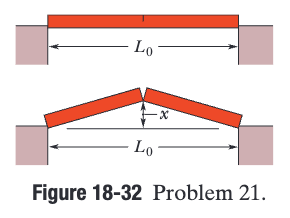
\includegraphics[width=0.5\textwidth]{picture_18-32.png} 
            % \label{fig:wrapfig}
        \end{wrapfigure}
        As a result of a temperature rise of 32 \unit{\celsius}, a bar with a crack at its center buckles upward (Fig. 18-32). The fixed distance $L_0$ is $3.77 \unit{\meter}$ and the coefficient of linear expansion of the bar is $25 \times 10^{-6}/\unit{\celsius}$. Find the rise x of the center.

        \subsection{Solution}
            We first find the final total length of the bar given the initial length.
            \begin{align}
                \Delta L &= L_0 \alpha \Delta T\\
                    &=  (3.77 \unit{\meter}) (25 \times 10^{-6}/\unit{\celsius}) (32 \unit{\celsius})\\
                    &=  3.016 \times 10^{-3} \unit{\meter}\\
                L_f &=  L_0 + \Delta L
                    =   3.77 \unit{\meter} + 3.016 \times 10^{-3} \unit{\meter}\\
                    &=  3.773016 \unit{\meter}
            \end{align}

            From this, we can use the Pythagoream Theorem to find the distance raised, bearing in mind that the values we use will be only half the magnitude of the values we found or know.
            \begin{align}
                x   &=  \sqrt{\left(\frac{3.773016}{2}\right)^2 - \left(\frac{3.77}{2}\right)^2}\\
                    &=  \sqrt{1.886508^2 - 1.885^2}\\
                    &=  \sqrt{5.69 \times 10^{-3} \unit{\meter^2}}
                    =   \boxed{0.0754 \unit{\meter}}
            \end{align}

    \pagebreak
    \section{Problem 23}
        A small electric immersion heater is used to heat 100 g of water for a cup of instant coffee. 
        The heater is labeled “200 watts” (it converts electrical energy to thermal energy at this rate). 
        Calculate the time required to bring all this water from 23.0\unit{\celsius} to 100\unit{\celsius}, ignoring any heat losses.

        \subsection{Solution}
            We have a formula for the heat transfered from the temperature.
            \begin{align}
                Q   &=  cm \Delta T
            \end{align}

            This has thermal energy in units of joules (\unit{\joule}).
            We can divide both by time to get the power (in units of watts (\unit{\joule/\second})) on the left side.
            \begin{align}
                \frac{Q}{t} &=  \frac{cm \Delta T}{t}\\
                P   &=  \frac{cm \Delta T}{t}
            \end{align}

            We can solve for the time.
            Recall the known mass and change in temperature, as well as the specific heat of water in \unit{\frac{\joule}{\kilo\gram\cdot\kelvin}}.
            \begin{align}
                t   &=  \frac{cm \Delta T}{P}\\
                    &=  \frac{\left( 4187\unit{\frac{\joule}{\kilo\gram\cdot\kelvin}} \right) \left( 0.1 \unit{\kilo\gram} \right) \left( 77 \unit{\kelvin} \right)}{200 \unit{\watt}}\\
                    &=  \frac{32239.9 \unit{\joule}}{200 \unit{\watt}}
                    =   \boxed{161.1995 \unit{\second} \approx 162 \unit{\second}}
            \end{align}

            Slight differences can be chocked up to sigfigs. 

    \pagebreak
    \section{Problem 25}
        A certain diet doctor encourages people to diet by drinking ice water. 
        His theory is that the body must burn off enough fat to raise the temperature of the water from 0.00°C to the body temperature of 37.0°C. 
        How many liters of ice water would have to be consumed to burn off 454 g (about 1 lb) of fat, assuming that burning this much fat requires 3500 Cal be transferred to the ice water? 
        Why is it not advisable to follow this diet? (One liter = $10^3 \unit{\centi\meter^3}$. 
        The density of water is $1.00 \unit{g/\centi\meter^3}$.)

        \subsection{Solution}
            We have a formula for this. 
            \begin{align}
                Q   &=  cm \Delta T
            \end{align}

            If we can find the mass of water required, we can find the volume given our known unit conversions, so we can isolate for that.
            \begin{gather}
                m   =   \frac{Q}{c \Delta T}
            \end{gather}

            The specific heat in this instance will be the specific heat of water ($c = 1 \unit{\frac{\calorie}{\gram\cdot\kelvin}} = 10^{-3} \unit{\frac{\Calorie}{\gram\cdot\kelvin}}$). 
            The change in temperature is 37.0\unit{\celsius}, which has identical magntude in Kelvin (\unit{K}). 
            \begin{align}
                m   &=  \frac{Q}{c \Delta T}
                    =   \frac{3500\unit{\Calorie}}{\left( 10^{-3} \unit{\frac{\Calorie}{\gram\cdot\kelvin}} \right) \left( 37.0 \unit{\kelvin} \right)}\\
                    &=  94594.6 \unit{\gram} * 1 \unit{\frac{\centi\meter^3}{\gram}} * 10^{-3} \unit{\frac{\liter}{\centi\meter^3}}\\
                    &=  \boxed{94.6 \unit{\liter}}
            \end{align}

            This requires drinking a \textit{lot} of ice water, about 47 and a half bottles of ice water per day. 
            I would not recommend it because it would take so long and would be so inefficient. 

    \pagebreak
    \section{Problem 27}
        Calculate the minimum amount of energy, in joules, required to completely melt 130 g of silver initially at 15.0\unit{\celsius}.

        \subsection{Solution}
        The amount of energy required for $130 \unit{\gram}$ of silver (melting point 1235 \unit{\kelvin}; $L_F = 105 \unit{\kilo\joule/\kilo\gram}$) can be separated into two parts: the energy necessary to heat it to melting temperature and the energy necessary to melt it at said temperature.
        \begin{align}
            E_\Sigma    &=  Q_{heat} + Q_{melt}
                =   cm\Delta T + Lm
        \end{align}

        Given these equations, we can calculate the total energy required.
        The specific heat of elemental solid silver is $236 \unit{\frac{\joule}{\kilo\gram\cdot\kelvin}}$.
        \begin{align}
            \Delta T    &=  1235 \unit{\kelvin} - 15.0 \unit{\celsius}
                =   1235 \unit{\kelvin} - 288.15 \unit{\kelvin}
                =   946.85 \unit{\kelvin}\\
            E_\Sigma    &=  \left( 236 \unit{\frac{\joule}{\kilo\gram\cdot\kelvin}} \right) (0.130 \unit{\kilo\gram}) (946.85 \unit{\kelvin}) + \left( 105 \unit{\frac{\joule}{\gram}} \right) \left( 130 \unit{\gram} \right)\\
                &=  29049.358 \unit{\joule} + 13650 \unit{joule}
                =   \boxed{42699.358 \unit{\joule} \approx 42700 \unit{\joule}}
        \end{align}

    \pagebreak
    \section{Problem 31}
        What mass of steam at 100\unit{\celsius} must be mixed with 150\unit{\gram} of ice at its melting point, in a thermally insulated container, to produce liquid water at 50\unit{\celsius}?

        \subsection{Solution}
        We can first calculate the amount of energy necessary for the ice to melt and heat to 50\unit{\celsius}. 
        \begin{align}
            Q   &=  cm \Delta T + Lm\\
                &=  \left( 4187 \unit{\frac{\joule}{\kilo\gram\cdot\kelvin}} \right) (0.15 \unit{\kilo\gram}) (50 \unit{\kelvin}) + (333 \unit{\joule/\gram}) (150 \unit{\gram})\\
                &=  31402.5 \unit{\joule} + 49950 \unit{\joule}
                =   81352.5 \unit{\joule}
        \end{align}

        This would be equal to the required energy from the steam to turn into liquid water at 50\unit{\celsius}.
        We can set up the same formula as above for the steam.
        \begin{gather}
            81352.5 \unit{\joule}   =   cm\Delta T + Lm = m(c\Delta T + L)\\
            \begin{align}
                m   &=  \frac{81352.5 \unit{\joule}}{c\Delta T + L}
                    =   \frac{81352.5 \unit{\joule}}{\left( 4187 \unit{\frac{\joule}{\kilo\gram\cdot\kelvin}} \right)(50\unit{\kelvin}) + 2256 \times 10^{3} \unit{\frac{\joule}{\kilo\gram}} }\\
                    &=  \frac{81352.5 \unit{\joule}}{ 209350 \unit{\frac{\joule}{\kilo\gram}} + 2256 \times 10^{3} \unit{\frac{\joule}{\kilo\gram}} }\\
                    &=  \frac{81352.5}{2465350} \unit{\kilo\gram}
            \end{align}\\
            m   =   \boxed{0.033 \unit{\kilo\gram} = 33 \unit{\gram}}
        \end{gather}

    \pagebreak
    \section{Problem 37}
        A person makes a quantity of iced tea by mixing 500\unit{\gram} of hot tea (essentially water) with an equal mass of ice at its melting point. 
        Assume the mixture has negligible energy exchanges with its environment. 
        If the tea's initial temperature is $T_i = 90\unit{\celsius}$, when thermal equilibrium is reached what are (a) the mixture's temperature $T_f$ and (b) the remaining mass $m_f$ of ice? If $T_i$ = 70°C, when thermal equilibrium is reached what are (c) $T_f$ and (d) $m_f$?

        \subsection{Solution (a)}
            First, we can calculate the energy that the tea have to would release to reduce its temperature to 0\unit{\celsius}, at which point it would start freezing if it released any more energy. 
            \begin{align}
                \Delta T    &=  0 \unit{\celsius} - 90 \unit{\celsius} = -90 \unit{\celsius}\\
                Q   &=  cm\Delta T\\
                    &=  \left( 4187 \unit{\frac{\joule}{\kilo\gram\cdot\kelvin}} \right) (0.5 \unit{\kilo\gram}) (-90 \unit{\celsius})\\
                    &=  -188415 \unit{\joule}
            \end{align}

            Next, we can calculate the amount of energy that would be absorbed by the ice completely melting.
            \begin{align}
                Q   &=  m L_F
                    =   \left( 333 \times 10^3 \unit{\joule/\kilo\gram} \right) \left( 0.5 \unit{\kilo\gram} \right)\\
                    &=  166500 \unit{\joule}
            \end{align}

            The magnitude of released energy is greater than the magnitude of absorbed energy, so all the ice will melt.
            To achieve thermal equilibrium, the energy absorbed by the ice would have to be equal to the energy released by the tea.
            We can find this by taking the average of the two quantities of energy found.
            From that, we can find the change in temperature of the water until it reaches thermal equilibrium.
            \begin{align}
                \frac{188415 + 166500}{2}   &=  177457.5\unit{\joule}   =   Q\\
                \Delta T    &=  \frac{Q}{cm}
                    =   \frac{-177457.5\unit{\joule}}{\left( 4187 \unit{\frac{\joule}{\kilo\gram\cdot\kelvin}} \right) (0.5 \unit{\kilo\gram})}
                    =   -84.766 \unit{\celsius}
            \end{align}

            This we can add to the initial temperature to find the final temperature.
            \begin{gather}
                T_f = T_i + \Delta T = 90 \unit{\celsius} - 84.766 \unit{\celsius} = \boxed{5.2 \unit{\celsius}}
            \end{gather}

        \subsection{Solution (b)}
            As established, all the ice melts, so $m_f = \boxed{0\unit{\gram}}$. 

        \subsection{Solution (c)}
            The ice would take the same amount of energy to melt, so $Q_{ice} = 166500 \unit{\joule}$.
            Knowing this, we should calculate the amount of energy to reduce all the tea to $0\unit{\celsius}$. 
            \begin{align}
                \Delta T    &=  0 \unit{\celsius} - 70 \unit{\celsius} = -70 \unit{\celsius}\\
                Q   &=  cm\Delta T\\
                    &=  \left( 4187 \unit{\frac{\joule}{\kilo\gram\cdot\kelvin}} \right) (0.5 \unit{\kilo\gram}) (-70 \unit{\celsius})\\
                    &=  -146545 \unit{\joule}
            \end{align}

            The magnitude of absorbed energy is greater than the magnitude of released energy, so less than all the ice will melt but all the water will reach \boxed{0\unit{\celsius}}.

        \subsection{Solution (d)}
            To achieve thermal equilibrium, the energy absorbed by the ice would have to be equal to the energy released by the tea.
            We can find this by taking the average of the two quantities of energy found.
            From that, we can find the lost mass of the ice when it reaches thermal equilibrium.
            \begin{align}
                \frac{146545 + 166500}{2}   &=  156522.5\unit{\joule}   =   Q\\
                Q   &=  m L_F\\
                m   &=  \frac{Q}{L_F}
                    =   \frac{156522.5\unit{\joule}}{333 \times 10^3 \unit{\joule/\kilo\gram}}\\
                    &=  0.47 \unit{\kilo\gram}
            \end{align}

            Subtract this from the total mass of the ice to find the final mass of ice not melted.
            \begin{equation}
                m_f =   0.5 \unit{\kilo\gram} - 0.47 \unit{\kilo\gram}  =   \boxed{0.03 \unit{\kilo\gram}}
            \end{equation}

        \subsection{Differential Equations Remark}
            This could be done with some differential equations.
            Presumably, the ice that is unfrozen would automatically start warming up and the full energy transfer would not be instantaneous, so we could set up a time variable and set up a function of the mass over time. 
            \begin{gather}
                Q   =   mL_F\\
                \dv{Q}{t} = \dv{m}{t} L_F
            \end{gather}


    \pagebreak
    \section{Problem 41}
        (a) Two 50 g ice cubes are dropped into 200\unit{\gram} of water in a thermally insulated container. 
        If the water is initially at 25\unit{\celsius}, and the ice comes directly from a freezer at -15\unit{\celsius}, what is the final temperature at thermal equilibrium? 
        (b) What is the final temperature if only one ice cube is used?
    
        \subsection{Solution}

    \pagebreak
    \section{Problem 43}
        \begin{wrapfigure}{r}{0.25\textwidth}
            \vspace{-30pt}
            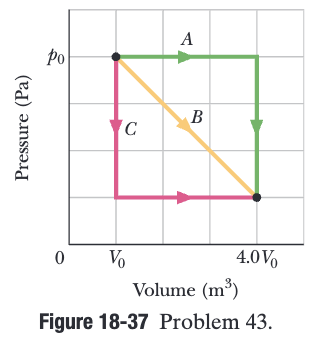
\includegraphics[width=0.25\textwidth]{picture_18-37.png} 
            % \label{fig:wrapfig}
        \end{wrapfigure}
        In Fig. 18-37, a gas sample expands from $V_0$ to $4.0 V_0$ while its pressure decreases from $p_0$ to $p_0/4.0$. 
        If $V_0 = 1.0 m^3$ and $p_0 = 40 \unit{\pascal}$, how much work is done by the gas if its pressure changes with volume via (a) path A, (b) path B, and (c) path C?

        \subsection{Solution}

    \pagebreak
    \section{Problem 45}

    \subsection{Solution}

    \pagebreak
    \section{Problem 47}

    \subsection{Solution}

    \pagebreak
    \section{Problem 49}

    \subsection{Solution}

    \pagebreak
    \section{Problem 51}

    \subsection{Solution}

    \pagebreak
    \section{Problem 53}

    \subsection{Solution}

    \pagebreak
    \section{Problem 57}

    \subsection{Solution}

    \pagebreak
    \section{Problem 59}

    \subsection{Solution}

    \pagebreak
    \section{Problem 63}

    \subsection{Solution}

    \pagebreak
    \section{Problem 85}

    \subsection{Solution}

    \pagebreak
    \section{Problem 89}

    \subsection{Solution}

    \pagebreak
    \section{Problem 93}

    \subsection{Solution}

    \pagebreak
    \section{Problem 103}

    \subsection{Solution}

    \pagebreak
    \section{Problem 105}

    \subsection{Solution}

    \pagebreak

    \tableofcontents
\end{document}